\Class{Cleric}
{Without destruction, there is nothing to build.}{Credo of the fire cleric}

In a world without gods, spiritualism on Athas has unlocked the secrets of the raw forces of which the very planet is comprised: earth, air, fire, and water. However, other forces exist which seek to supplant them and rise to ascendancy in their place. These forces have taken up battle against the elements of creation on the element's own ground in the form of entropic perversions of the elements themselves: magma, rain, silt and sun.

\SpellcasterTable{The Cleric}{.5cm}{
1 & +0 & +2 & +0 & +2 & Pact, turn or rebuke undead & 3 & 1+1 &  &  &  &  &  &  &  &  \\
2 & +1 & +3 & +0 & +3 &  & 4 & 2+1 &  &  &  &  &  &  &  &  \\
3 & +2 & +3 & +1 & +3 &  & 4 & 2+1 & 1+1 &  &  &  &  &  &  &  \\
4 & +3 & +4 & +1 & +4 &  & 5 & 3+1 & 2+1 &  &  &  &  &  &  &  \\
5 & +3 & +4 & +1 & +4 &  & 5 & 3+1 & 2+1 & 1+1 &  &  &  &  &  &  \\
6 & +4 & +5 & +2 & +5 &  & 5 & 3+1 & 3+1 & 2+1 &  &  &  &  &  &  \\
7 & +5 & +5 & +2 & +5 &  & 6 & 4+1 & 3+1 & 2+1 & 1+1 &  &  &  &  &  \\
8 & +6/+1 & +6 & +2 & +6 &  & 6 & 4+1 & 3+1 & 3+1 & 2+1 &  &  &  &  &  \\
9 & +6/+1 & +6 & +3 & +6 &  & 6 & 4+1 & 4+1 & 3+1 & 2+1 & 1+1 &  &  &  &  \\
10 & +7/+2 & +7 & +3 & +7 &  & 6 & 4+1 & 4+1 & 3+1 & 3+1 & 2+1 &  &  &  &  \\
11 & +8/+3 & +7 & +3 & +7 &  & 6 & 5+1 & 4+1 & 4+1 & 3+1 & 2+1 & 1+1 &  &  &  \\
12 & +9/+4 & +8 & +4 & +8 &  & 6 & 5+1 & 4+1 & 4+1 & 3+1 & 3+1 & 2+1 &  &  &  \\
13 & +9/+4 & +8 & +4 & +8 &  & 6 & 5+1 & 5+1 & 4+1 & 4+1 & 3+1 & 2+1 & 1+1 &  &  \\
14 & +10/+5 & +9 & +4 & +9 &  & 6 & 5+1 & 5+1 & 4+1 & 4+1 & 3+1 & 3+1 & 2+1 &  &  \\
15 & +11/+6/+1 & +9 & +5 & +9 &  & 6 & 5+1 & 5+1 & 5+1 & 4+1 & 4+1 & 3+1 & 2+1 & 1+1 &  \\
16 & +12/+7/+2 & +10 & +5 & +10 &  & 6 & 5+1 & 5+1 & 5+1 & 4+1 & 4+1 & 3+1 & 3+1 & 2+1 &  \\
17 & +12/+7/+2 & +10 & +5 & +10 &  & 6 & 5+1 & 5+1 & 5+1 & 5+1 & 4+1 & 4+1 & 3+1 & 2+1 & 1+1 \\
18 & +13/+8/+3 & +11 & +6 & +11 &  & 6 & 5+1 & 5+1 & 5+1 & 5+1 & 4+1 & 4+1 & 3+1 & 3+1 & 2+1 \\
19 & +14/+9/+4 & +11 & +6 & +11 &  & 6 & 5+1 & 5+1 & 5+1 & 5+1 & 5+1 & 4+1 & 4+1 & 3+1 & 2+1 \\
20 & +15/+10/+5 & +12 & +6 & +12 &  & 6 & 5+1 & 5+1 & 5+1 & 5+1 & 5+1 & 4+1 & 4+1 & 3+1 & 3+1}

\begin{figure}[t!]
\centering
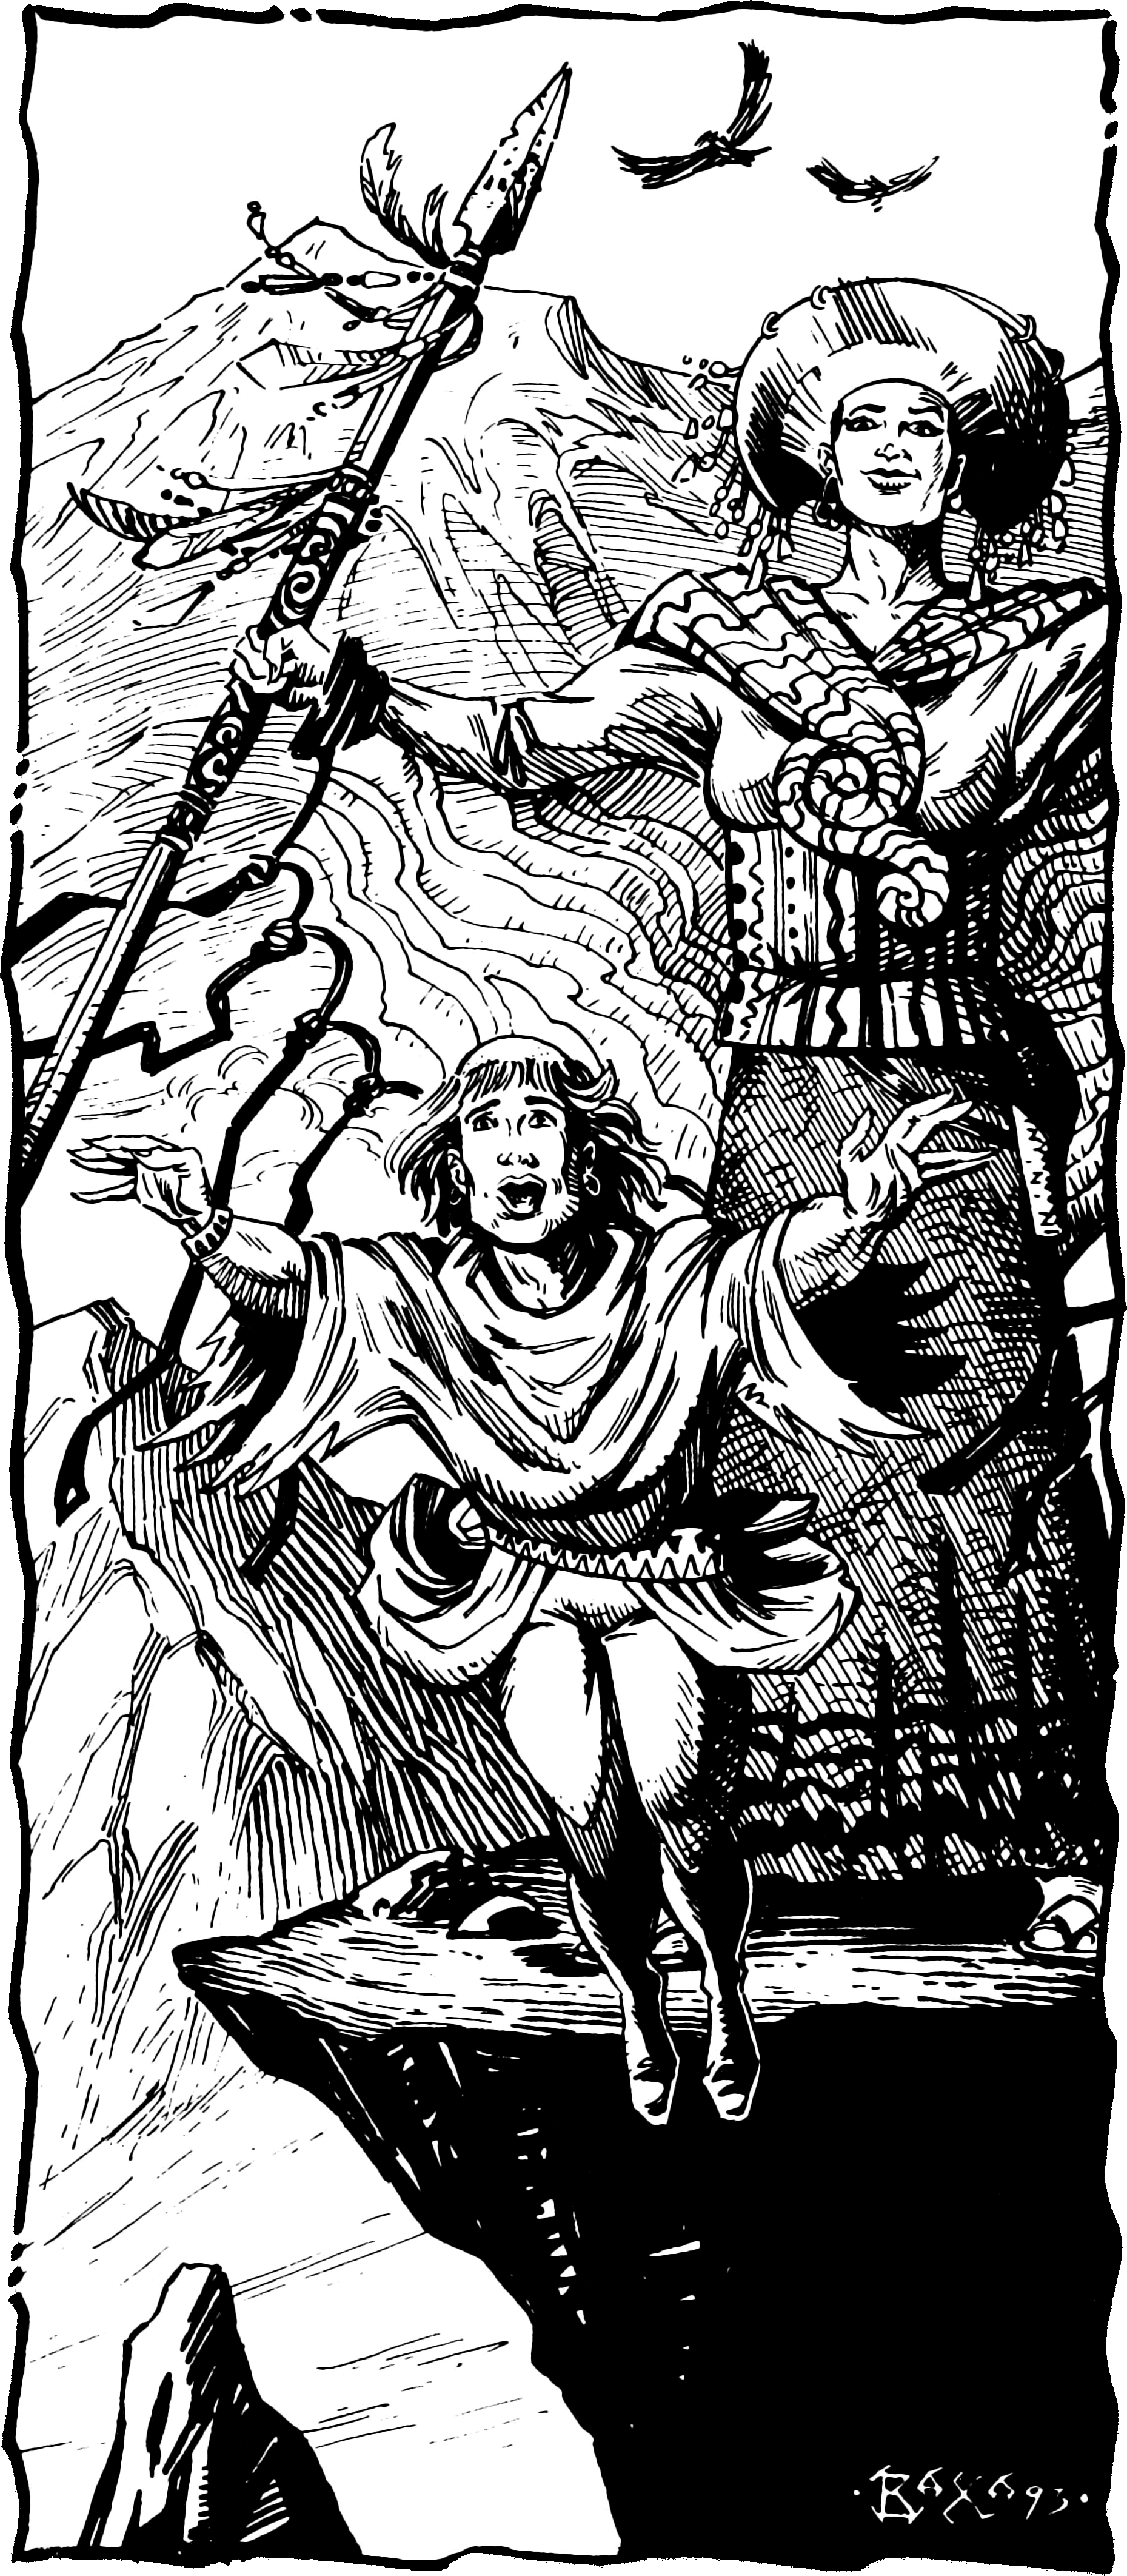
\includegraphics[width=\columnwidth]{images/cleric-1.png}
\end{figure}

\subsection{Making a Cleric}
Clerics are the masters of elemental forces; they possess unique supernatural abilities to direct and harness elemental energy, and cast elemental spells. All things are comprised of the four elements in some degree, thus clerics can use their elemental powers to heal or harm others. Due to their affinities with the elements, clerics possess a number of supernatural elemental abilities. Though dimly understood, there exists a connection between elemental forces and the nature of undeath. Clerics can turn away, control, or even destroy undead creatures. Athas is a dangerous world; this practicality dictates that clerics must be able to defend themselves capably. Clerics are trained to use simple weapons and, in some cases, martial weapons; they are also taught to wear and use armor, since wearing armor does not interfere with elemental spells as it does arcane spells.

\textbf{Races}: All races include clerics in their societies, though each race possesses different perspectives regarding what a cleric's role involves. As masters of myth and the elemental mysteries, most clerics hold a place of reverence within their respective societies. However, more than a few races have varying affinities for one element over another. Dwarves almost always become earth clerics, a connection they've shared since before they were driven from their halls under the mountains. Dwarven determination and obsessive dedication matches perfectly with the enduring earth. Elves most often revere water, fire, or the winds; as nomads, they seldom feel a deep-seated affinity for the land. Thri-kreen are known to ally with all elements to the exclusion of fire. This seems to stem from a mistrust of flame, which is common in many kreen.

\textbf{Alignment}: Attaining the abilities of a true servant of the elements requires a deep understanding of the chosen kind of element of paraelement. An aspiring cleric must make a study of the element's typical personality and role; opens the door to the element's power. Thus, Athasians clerics align their morals to suit the traits of the element to which they dedicate themselves.

\subsection{Game Rule Information}

\textbf{Hit Die}: d8.

\subsubsection{Class Skills}
\skill{Concentration} (Con), \skill{Craft} (Int), \skill{Diplomacy} (Cha), \skill{Heal} (Wis), \skill{Knowledge} (arcana) (Int), \skill{Knowledge} (history) (Int), \skill{Knowledge} (religion) (Int), \skill{Knowledge} (the planes) (Int), \skill{Profession} (Wis), and \skill{Spellcraft} (Int).

\textbf{Skill Points per Level}: 2 + Int modifier ($\times4$ at 1st level).

\subsubsection{Class Features}
\textbf{Weapon and Armor Proficiency}: Clerics are proficient with light armor and all simple weapons.

\textbf{Aura (Ex)}: A cleric has a particularly powerful aura corresponding to the her alignment (see the \spell{detect evil} spell for details).

\textbf{Spells}: A cleric casts divine spells, which are drawn from the cleric spell list. However, his alignment may restrict him from casting certain spells opposed to his moral or ethical beliefs; see Chaotic, Evil, Good, and Lawful Spells, below. A cleric must choose and prepare his spells in advance (see below).

To prepare or cast a spell, a cleric must have a Wisdom score equal to at least 10 + the spell level. The Difficulty Class for a saving throw against a cleric's spell is 10 + the spell level + the cleric's Wisdom modifier.

Like other spellcasters, a cleric can cast only a certain number of spells of each spell level per day. His base daily spell allotment is given on \tabref{The Cleric}. In addition, he receives bonus spells per day if he has a high Wisdom score. A cleric also gets one domain spell of each spell level he can cast, starting at 1st level. When a cleric prepares a spell in a domain spell slot, it must come from one of his domains (see Pact, below).

Clerics meditate or pray for their spells. Each cleric must choose a time at which he must spend 1 hour each day in quiet contemplation or supplication to regain his daily allotment of spells. Time spent resting has no effect on whether a cleric can prepare spells. A cleric may prepare and cast any spell on the cleric spell list or on his domains spell lists, provided that he can cast spells of that level, but he must choose which spells to prepare during his daily meditation.

\BigTablePair{Athasian Elements and Paraelements}{llXlll} {
& \tableheader Type & \tableheader Class Skill & \tableheader Domains & \tableheader Energy Type & \tableheader Worshipers\\
\textit{Air} & Element & \skill{Survival} & Air, Forecasting, Freedom & Sonic & Aarakocra, elves\\
\textit{Earth} & Element & \skill{Knowledge} (nature) & Agriculture, Cycle, Earth & Acid & Dwarves, muls\\
\textit{Fire} & Element & \skill{Knowledge} (architecture and engineering) & Cleansing, Fire, Wrath & Fire & Dwarves, ssurrans\\
\textit{Water} & Element & \skill{Knowledge} (geography) & Purity, Replenishment, Water & Acid & Half-elves, lizardfolk\\
\textit{Magma} & Paraelement & \skill{Climb} & Drought, Magma & Fire & Ssurrans\\
\textit{Rain} & Paraelement & \skill{Survival} & Growth, Rain & Electricity & Drajis\\
\textit{Silt} & Paraelement & \skill{Balance} & Silt, Thirst & Acid & Giants, silt runners\\
\textit{Sun} & Paraelement & \skill{Spot} & Mirage, Sun & Fire & Aarakocra\\
}

% \textbf{Elements, Domains, and Domain Spells}: A cleric's element influences what magic he can perform, his values, and how others see him. A cleric chooses two domains from among those belonging to his element.

% Each domain gives the cleric access to a domain spell at each spell level he can cast, from 1st on up, as well as a granted power. The cleric gets the granted powers of both the domains selected.

% With access to two domain spells at a given spell level, a cleric prepares one or the other each day in his domain spell slot. If a domain spell is not on the cleric spell list, a cleric can prepare it only in his domain spell slot.

\textbf{Pact}: Clerics forge a pact of servitude with elemental beings in exchange of divine powers. Each element and paraelement requires different duties and give different set of powers. They give an additional class skill for the cleric, and grant access to two domains from a select list (see \tabref{Athasian Elements and Paraelements}).

Each domain gives the cleric access to a domain spell at each spell level he can cast, from 1st on up, as well as a granted power. The cleric gets the granted powers of both the domains selected.

With access to two domain spells at a given spell level, a cleric prepares one or the other each day in his domain spell slot. If a domain spell is not on the cleric spell list, a cleric can prepare it only in his domain spell slot.

\textbf{Spontaneous Casting}: A good cleric can channel stored spell energy into healing spells that the cleric did not prepare ahead of time. The cleric can ``lose'' any prepared spell that is not a domain spell in order to cast any cure spell of the same spell level or lower (a cure spell is any spell with ``cure'' in its name).

An evil cleric, can't convert prepared spells to cure spells but can convert them to inflict spells (an inflict spell is one with ``inflict'' in its name).

A cleric who is neither good nor evil can convert spells to either cure spells or inflict spells (player's choice). Once the player makes this choice, it cannot be reversed. This choice also determines whether the cleric turns or commands undead.

\textbf{Chaotic, Evil, Good, and Lawful Spells}: A cleric can't cast spells of an alignment opposed to his own. Spells associated with particular alignments are indicated by the chaos, evil, good, and law descriptors in their spell descriptions.

\textbf{Turn or Rebuke Undead (Su)}: Any cleric, regardless of alignment, has the power to affect undead creatures by channeling the power of his faith through his holy (or unholy) symbol.

A good cleric can turn or destroy undead creatures. An evil cleric instead rebukes or commands such creatures. A neutral cleric must choose whether his turning ability functions as that of a good cleric or an evil cleric. Once this choice is made, it cannot be reversed. This decision also determines whether the cleric can cast spontaneous cure or inflict spells.

A cleric's worshiped element or paraelement has no impact on your ability to turn or rebuke undead. However, all elements and paraelements consider the undead to be a violation of the natural order of things. While evil clerics are free to control undead, they are expected to eventually destroy them.

A cleric may attempt to turn undead a number of times per day equal to 3 + his Charisma modifier. A cleric with 5 or more ranks in \skill{Knowledge} (religion) gets a +2 bonus on turning checks against undead.

\subsubsection{Duties}
To fulfill the pact, a cleric must live up to the pact made with their patron.

% For more information on what are the specific duties of each element, see \chapref{Magic}.
\textbf{Elements}: Elementals realize the balance needed to survive and their pact reflects their wish for preservation. Every elemental cleric must oppose defilers, although some are more zealous than others.

\textit{Air}: Air clerics must
	(i) actively oppose slavery and unfair imprisonment;
	(ii) preserve earth and water.

They loathe restriction in their movements, personalities, beliefs, practices, and clothing, and they rebel against any attempts to impose limitations. And by preserving earth and water, the elementals hope that the mighty forests will return to shelter the planet from the harsh sun, and that the raging oceans will once again fill the great silt basins. Only then will they regain the unbridled freedom they once knew.

\textit{Earth}: Earth clerics must
	(i) actively oppose defilers. They may not travel or work with a known defiler, nor can they allow a defiler to cast a spell in their presence;
	(ii) teach the nature of the cycle of life;
	(iii) teach proper agricultural techniques.

Earth clerics don't usually seek revenge in the same way that druids do, for their opposition to the defilers is purely defensive. When they are up against a known defiler, earth clerics are far more likely to incite others to fight for them, while they continue their silent opposition in the background.

\textit{Fire}: Fire clerics must
	(i) encourage the growth of cities, forests, and fields;
	(ii) actively oppose sorcerer-monarchs and defilers.

A large part of the pact is dedicated to the defeat sorcerer-kings and all defilers. This is a goal they share with the druids, but the priests of fire are too eccentric to form one long, lasting relationships with the members of that elusive order. A frontal assault wielding the power of the inferno is their usual tactic.

\textit{Water}: Water clerics must
	(i) give water and aid to anyone in need. The only exception being defilers;
	(ii) protect and preserve any remaining water sources from any danger, including defilers;
	(iii) teach how to best use water supplies.

It is the duty of water clerics to give water and aid to any in need, of any alignment, of any nature. The only exceptions are those who criminally waste water. Water clerics should never allow a defiler to cast a spell near a water source, nor permit a forest or any other moisture producing area be destroyed. They must teach these ideas to any who will listen.

\begin{figure}[b!]
\centering
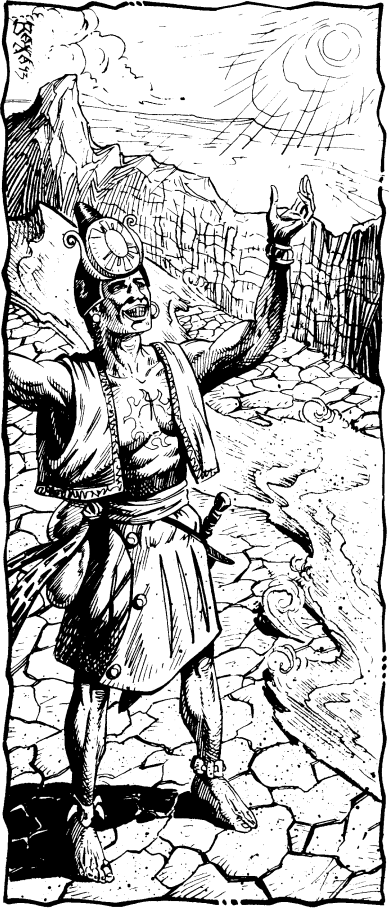
\includegraphics[width=\columnwidth]{images/cleric-3.png}
\end{figure}

\textbf{Paraelements}: Paraelementals wish only to grow their domains to the extent of Athas itself, even if it destroys the planet in the process. Their greedy demands are usually met with mad clerics that take these tasks to the extreme.

\textit{Magma}: Magma clerics must
	(i) keep magma heated;
	(ii) destroy all moisture sources near magma, such as forests and lakes.

Magma demands only that its clerics encourage its growth. Usually, the only things that retard magma are water, rain, or lack of sufficient fuel to maintain the tremendous heat magma requires. Magma clerics have been known to destroy forests in order to prevent rainfall, and then to feed the branches and logs into rolling rivers of lava.

\textit{Rain}: Rain clerics must
	(i) protect forests and water reserves;
	(ii) plant new forests.

The creatures of rain wish only to return their patron's cool caresses to Athas. To do this, the forests that protect and hold the world's water must return.

\textit{Silt}: Silt clerics must
	(i) transform earth into silt;
	(ii) bury all moisture sources into silt, such as plants and pools of water.

The beings who dwell on the Paraelemental Plane of Silt demand only one thing from their mortal minions---the growing tides of silt must continue to expand, eventually to wash over the entire planet. It is said that rare silt clerics fulfill their pacts by working in small stages or by toiling in areas already ruined for any other purposes. Others sometimes pose as earth clerics to teach farming methods that ruin the soil.

\textit{Sun}: Sun clerics must
	(i) make all gatherings under the sun;
	(ii) remove any shade that blocks the sun.

Sun priests must help eliminate anything that filters and weakens the rays of the sun and remove any other obstructions that would dare defy its radiant omnipotence.

\subsubsection{Ex-Clerics}
When a cleric fails to fulfill their vows or encourages others to waste their patron's resources, the elemental powers will suspend their blessing upon the cleric for up to six days, depending on the severity. They lose all spells during this period.

A cleric that breaks their vows for a second time can no longer gain any new cleric levels, and lose all clerical spells and abilities until they atone (see the \spell{atonement} spell).

\subsection{Playing a Cleric}
The clerics of Athas are like the rare snows that blanket the highest peaks of the Ringing Mountains. Though the cascading flakes all seem the same, the pattern of each is as different as the faces of men are from muls. Indeed, clerics are like snowflakes, each preaching about preservation and the elements, but no two of them do it for the same reason. This makes these environmental warriors an extremely diverse and interesting class to play. Some are merely power-hungry, some seek revenge, and some are honestly struggling to save their dying planet and reverse the ancient environmental disaster.

You are a servant of your element, your goal in life is to expand its presence in Athas, and find your element's foes and destroy them with your cleansing element.

You adventure out of a desire to preach the words of your element, prove your worth and to destroy infidels who worship opposed elements.

\subsubsection{Religion}
Unlike clerics found on other worlds, elemental clerics do not generally congregate at temples or churches, nor do they participate in a uniform, organized religion. Each cleric's calling to the raw energy of the elements is personal, individual. Some clerics believe that, upon their initiation, they enter pacts with powerful beings, elemental lords, who grant powers to those who contract with them. Others believe that the elements are neither malevolent nor benevolent, but a tool to be used, or a force to be harnessed. Regardless, all clerics desire the preservation of their patron element, though the reasons for this are many and varied.

Clerics are found everywhere on Athas. Most common clerics are wanderers, who preach the concept of preservation with the hope of restoring Athas to a greener state. Wanderers are generally well received by those that dwell in the desert, such as villagers and slave tribes. They cure the sick and heal the wounded, sometimes even aiding in defeating local threats. Other clerics act as wardens of small, hidden shrines, which they hope creates a clearer channel to the elemental plane of worship, and fortifies their powers and spells. Tribal and primitive societies include shamans, who see to the spiritual needs of their groups, offering advice to the leaders and providing supernatural protection and offense. Lastly, some clerics stay in the cities, where they most commonly work against the sorcerer-kings and their templars. There they quietly preach the message of preservation to the citizenry, and even sometimes work with the Veiled Alliance.

\subsubsection{Other Classes}
In an adventuring party, the cleric often fills the role of advisor and protector. Clerics often possess an unshakable distrust of wizards and their arcane spells. Most clerics are well aware of the danger that sorcery represents to the dying planet, and watch those who wield such power carefully. Generally speaking, the elemental clerics are all on friendly terms with each other, recognizing an ancient pact made by their ancestors to put aside their differences in the opposition of Athas' destruction. However, clerics whose elements are diametrically opposed often clash regarding the means used in furthering their goals, and at times this has led to bloodshed.

\subsubsection{Combat}
Athasian clerics make use of the same general combat tactics as those described in the Player's Handbook---that is, stay back from melee and use your spells to either destroy your enemies or enhance your allies' abilities.

Your tactics on the battlefield depend largely on your element and domains chosen. Air clerics are not very offensive, but when needed they usually employ sonic attacks from the heights. Earth clerics believe the best defense is a good offense, but they also employ the strongest of metal weapons. Fire clerics are feared and unpredictable, appearing to thrive only when everything around them is being devoured by the fiery appetites of their patrons. Water clerics are usually healers, but they can be known to be meticulous in the cruelty of their vengeance when someone wantonly wastes water.

Don't neglect your ability to heal yourself or your allies, but don't burn through your spells early in an attempt to do so; make the most efficient use of your spells in battle, saving the healing until combat is over or it becomes absolutely necessary.

\subsubsection{Advancement}
Your first steps towards becoming a cleric were witnessing your element in action. After learning what your element could do, and that they could grant such powers into you, you dedicated yourself into serving your element. Your elemental pact marked the beginning of your journey and unlocked the first of many new abilities other creatures can only dream about.

You have only just begun your quest to become worthy of your element, and a lifetime of striving still lies ahead of you. If you truly want to serve your element the best you can, consider taking the elementalist prestige class (page 93).

\subsection{Starting Packages}
\subsubsection{The Defender}

Dwarf Earth Cleric

\textbf{Ability Scores}: Str 13, Dex 8, Con 16, Int 12, Wis 15, Cha 8.

\textbf{Skills}: \skill{Concentration}, \skill{Knowledge} (religion).

\textbf{Languages}: Common, Dwarven, Terran.

\textbf{Feat}: \feat{Disciplined}.

\textbf{Weapons}: Maul (1d12)

Bolas (1d4, 3 m).

\textbf{Armor}: Scale mail (+6 AC).

\textbf{Gear}: Spell component pouch, standard adventurer's kit, 45 cp.

\textbf{Class Features}: Channels positive energy; Cycle and Earth domains.

\textbf{Spells Prepared}: 1st---\spell{magic stone}$^D$, \spell{protection from evil}, \spell{shield of faith}; 0---\spell{create element}, \spell{detect element}, \spell{resistance}.

D: Domain spell.

\subsubsection{The Destroyer}

Human Magma Cleric

\textbf{Ability Scores}: Str 14, Dex 8, Con 13, Int 10, Wis 15, Cha 12.

\textbf{Skills}: \skill{Concentration}.

\textbf{Languages}: Common.

\textbf{Feat}: \feat{Combat Casting}, \feat{Elemental Might}.

\textbf{Weapons}: Heartpick (1d8/$\times$4).

\textbf{Armor}: Scale mail (+4 AC), heavy wooden shield (+2 AC).

\textbf{Gear}: Spell component pouch, standard adventurer's kit, 59 cp.

\textbf{Class Features}: Channels positive energy; Drought and Magma domains.

\textbf{Spells Prepared}: 1st---\spell{bless}, \spell{divine favor}, \spell{magic stone}$^{D}$; 0---\spell{create element}, \spell{resistance}, \spell{virtue}.

D: Domain spell.

\subsubsection{The Healer}

Pterran Water Cleric

\textbf{Ability Scores}: Str 14, Dex 10, Con 10, Int 8, Wis 17, Cha 15.

\textbf{Skills}: \skill{Concentration}, \skill{Diplomacy}, \skill{Heal}.

\textbf{Languages}: Saurian.

\textbf{Feat}: \feat{Skill Focus} (Heal).

\textbf{Weapons}: Longspear (1d8/$\times$3)

Net (3 m).

\textbf{Armor}: Scale mail (+4 AC).

\textbf{Gear}: Spell component pouch, standard adventurer's kit, 50 cp.

\textbf{Class Features}: Channels positive energy; Purity and Replenishment domains.

\textbf{Spells Prepared}: 1st---\spell{clear water}$^{D}$, \spell{protection from evil}, \spell{sanctuary}; 0---\spell{create element}, \spell{detect poison}, \spell{purify food and drink}.

D: Domain spell.

\subsection{Clerics on Athas}
\Quote{As for the elemental clerics, some say we are mad---driven insane by the chaotic beings we serve. But others see the gleam of patience in our eyes, and know that one day the clerics of Athas will throw off the yoke of oppression and return the flowing rivers and the sprawling forests to our withered lands.}{Jurgan, Urikite earth cleric}

Like the Athasian deserts, the elemental powers are neither benevolent nor malevolent, caring only that their natural forms are preserved in the material world. This is the source of their power, and the impending ecological collapse in Athas has created an unusual and dynamic power struggle on the elemental planes. The clerics of Athas are nothing but the pawns of this titanic struggle.

\subsubsection{Daily Life}

A cleric typically begins his day by finding a suitable locale where he can commune with his element and pray for the spells he desires. He then spends the rest of the day engaged in whatever task seems most important for advancing his element's goals while trying to avoid too much trouble. When not adventuring, clerics often spend their time seeking out scraps of information about the elemental planes and other clerics. The pursuit of such knowledge is often quite dangerous and can result in the cleric undertaking additional adventures.

\subsubsection{Notables}

The pursuit of his element's goals garners notoriety for a cleric, but it also can bring about his death of force him into exile. The Wanderer, famous for compiling the history and geography of Athas, is said to be an earth cleric. The sun cleric Caelum (page 285) became famous for leading his Dwarven army in their metal armor against the sorcerer-kings and helping re-imprisoning Rajaat back in to the Hollow.

\subsubsection{Organizations}

A cleric usually finds a role in an adventuring party or other organization that allows his free time to explore his divine abilities freely. Since no organization specifically caters to Athasian clerics, many find themselves in drastically different circumstances from those of their comrades.

Within the ranks of elemental clerics, prestige and influence is measured by the depth of their devotion to their element. The most highly admired are those who have further accomplished their element's pact and those who most wield elemental power. When two or more clerics come into conflict, they usually defer to the one with a greater knowledge of their element, relying on wisdom and experiences to provide a reasonable solution.

The elemental clerics are much more tightly tied to their temples than paraelemental ones. Because the elements are losing the battle against the paraelements, they cannot afford to be without staunch allies.

\subsubsection{NPC Reactions}

The reactions clerics receive from communities are directly tied to how those cultures regard their specific element. A silt cleric is viewed in a much friendlier manner near to the Sea of Silt than near the Forest Ridge, for example.

As a general rule of thumb, an NPC's attitude is one step nearer helpful for elemental clerics and one step nearer hostile for paraelemental clerics.

\subsubsection{Cleric Lore}

Characters with ranks in \skill{Knowledge} (religion) can research clerics to learn more about them. When a character makes a skill check, read or paraphrase the following, including the information from lower DCs.

\textbf{DC 10}: Clerics are divine spellcasters that serve the elemental powers.

\textbf{DC 15}: A cleric devotes himself to a particular kind of element gains power based on the element chosen. They can easily heal of harm those around him by channeling divine energy.

\textbf{DC 20}: Elemental clerics have forged a pact of sorts in order to fight the paraelement clerics and their quick expansion over Athas.
